\chapter{Recoil Correction}\label{appendix:ApendiceB}

To derive the corrections, we use a singleMuon sample for data and a DYJetsToLL for MC. For the $Z \rightarrow \mu \mu$ process we use the following selection:

In Data:
\begin{itemize}
\item
Trigger :  $\verb|HLT_IsoMu20_v* OR  HLT_IsoTkMu20_v*|$
\item
Good offline primary vertex
\item
$\pt >$ 25 GeV , $\left| \eta \right| <$ 2.4
\item
Tight muon ID
\item
Relative isolation with $\Delta \beta$ correction less than 0.15
\item
$ \Delta R(muon,muon) >$ 0.5
\item
60 $<$ $m_{Z}$ $<$ 120 GeV
\item
Opposite charge muons
\end{itemize}

In MC we apply the same selection, but in addition:
\begin{itemize}
\item
PU reweighting
\item
Muon Id/Iso and trigger scale factors
\item
JEC
\end{itemize}
Figure \ref{fig:METrecoil1} shows the main kinematic properties and recoil variables after the selection.
\newpage
\begin{figure}[!ht]
\begin{tabular}{cc}
  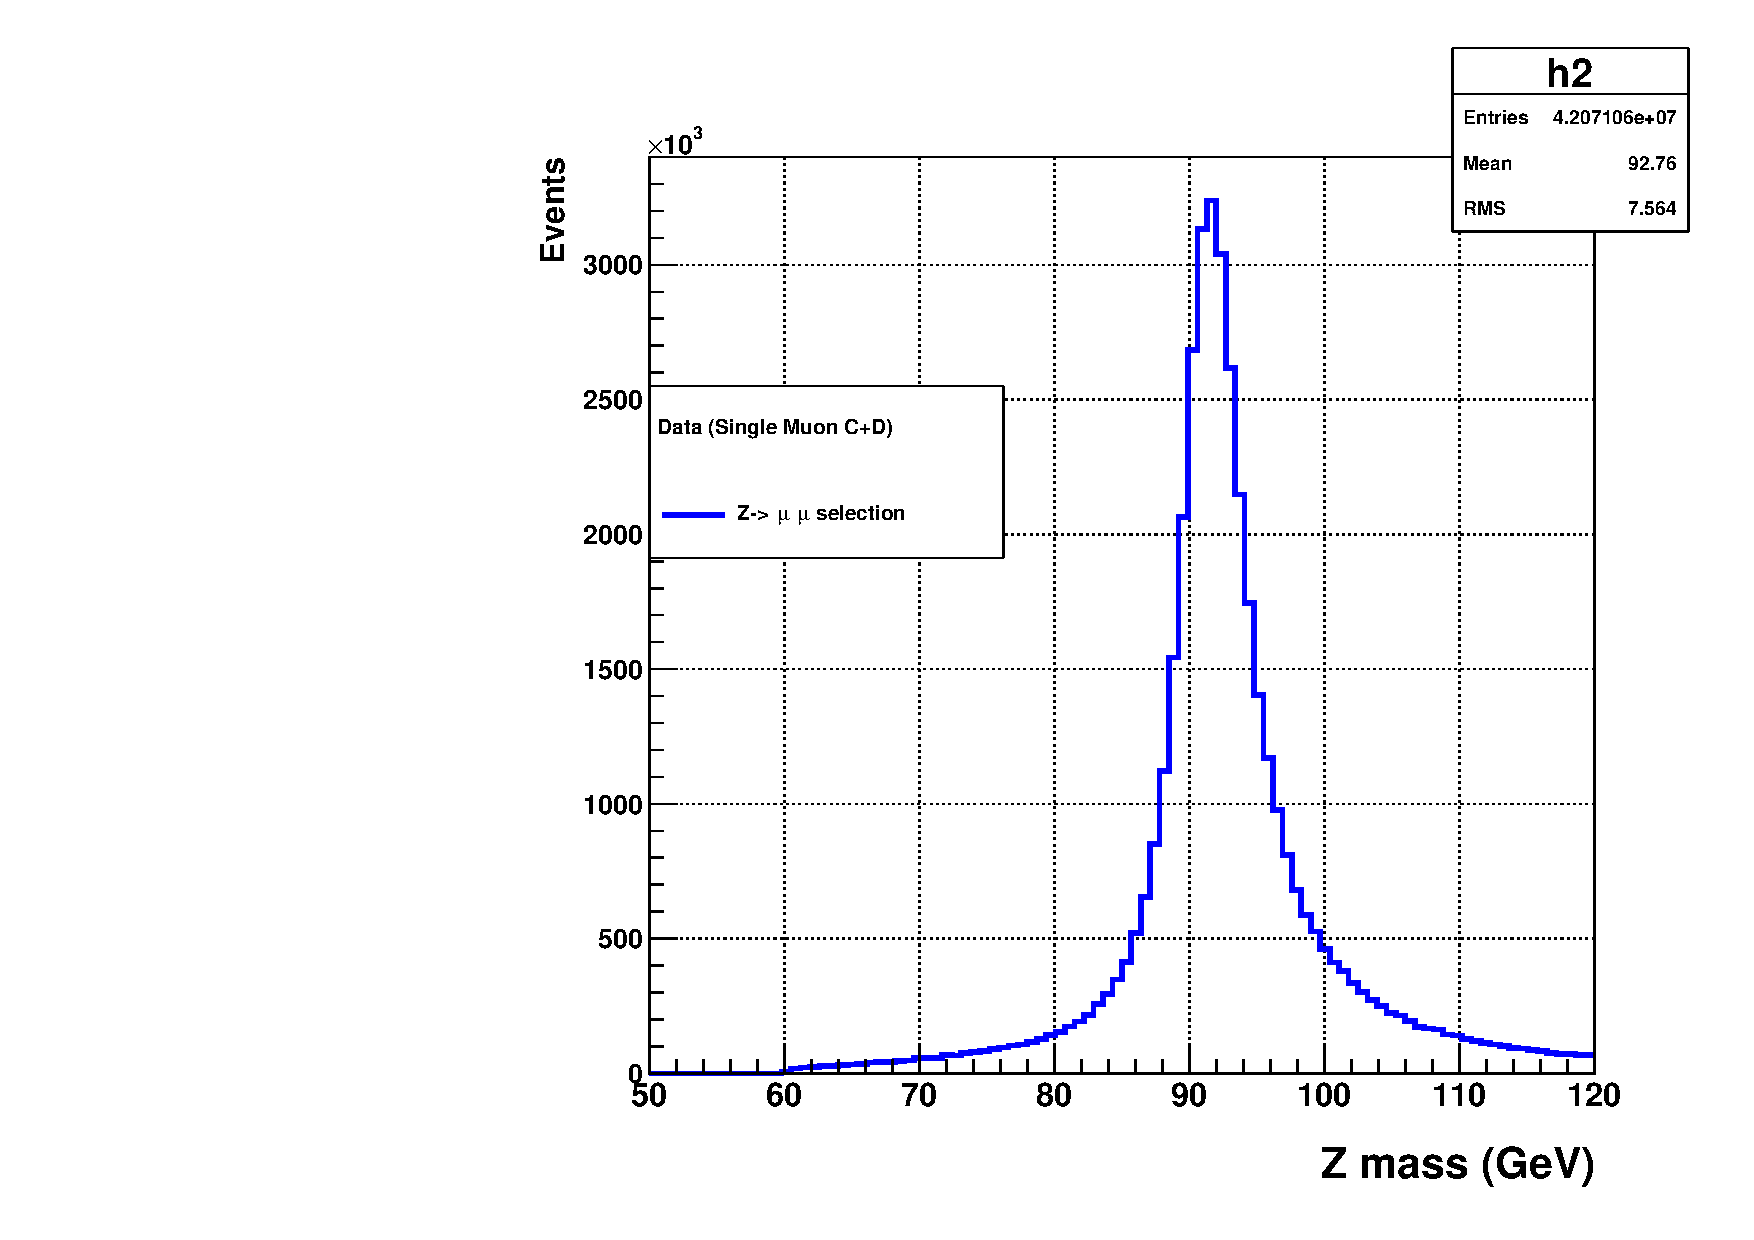
\includegraphics[width=180pt]{figuresARC/recoil/dileptonMass.pdf} &
  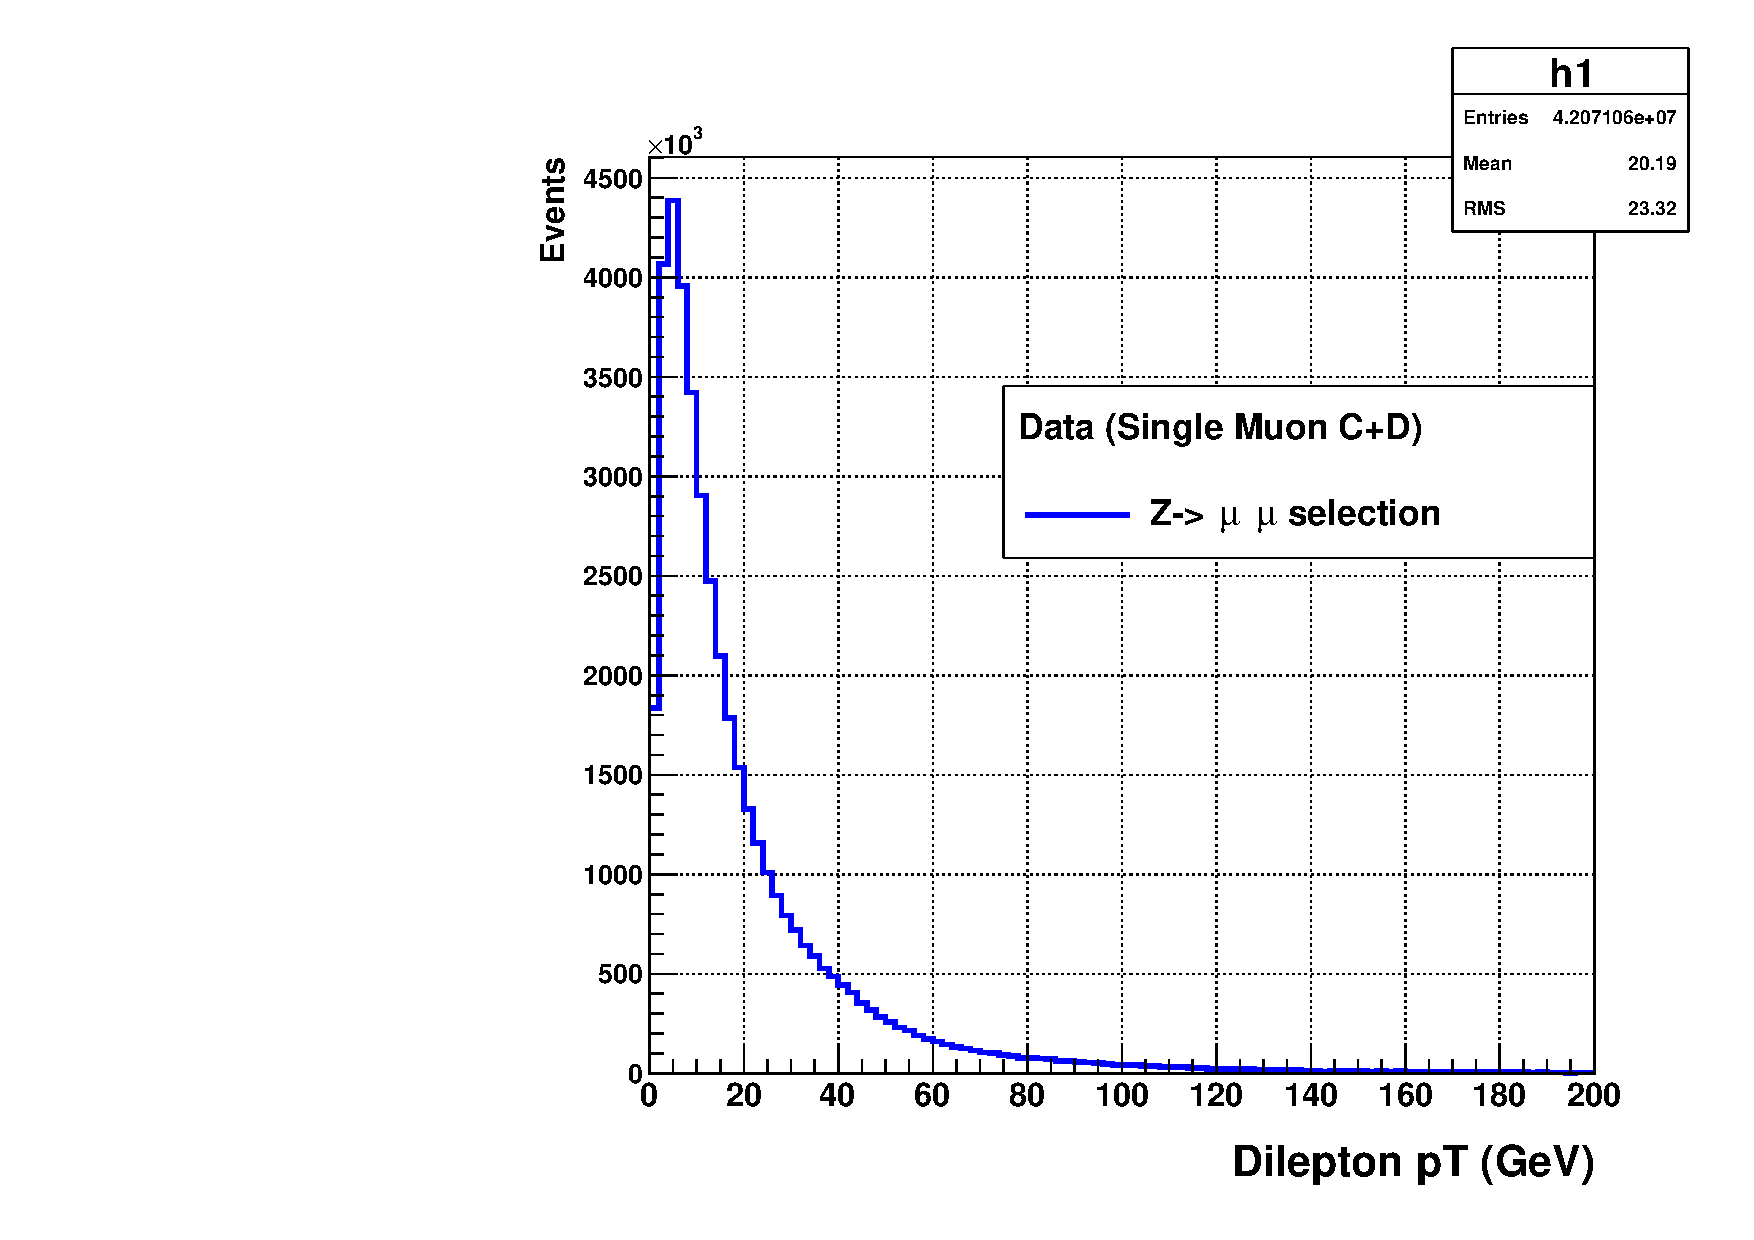
\includegraphics[width=180pt]{figuresARC/recoil/dileptonpt.pdf} \\
  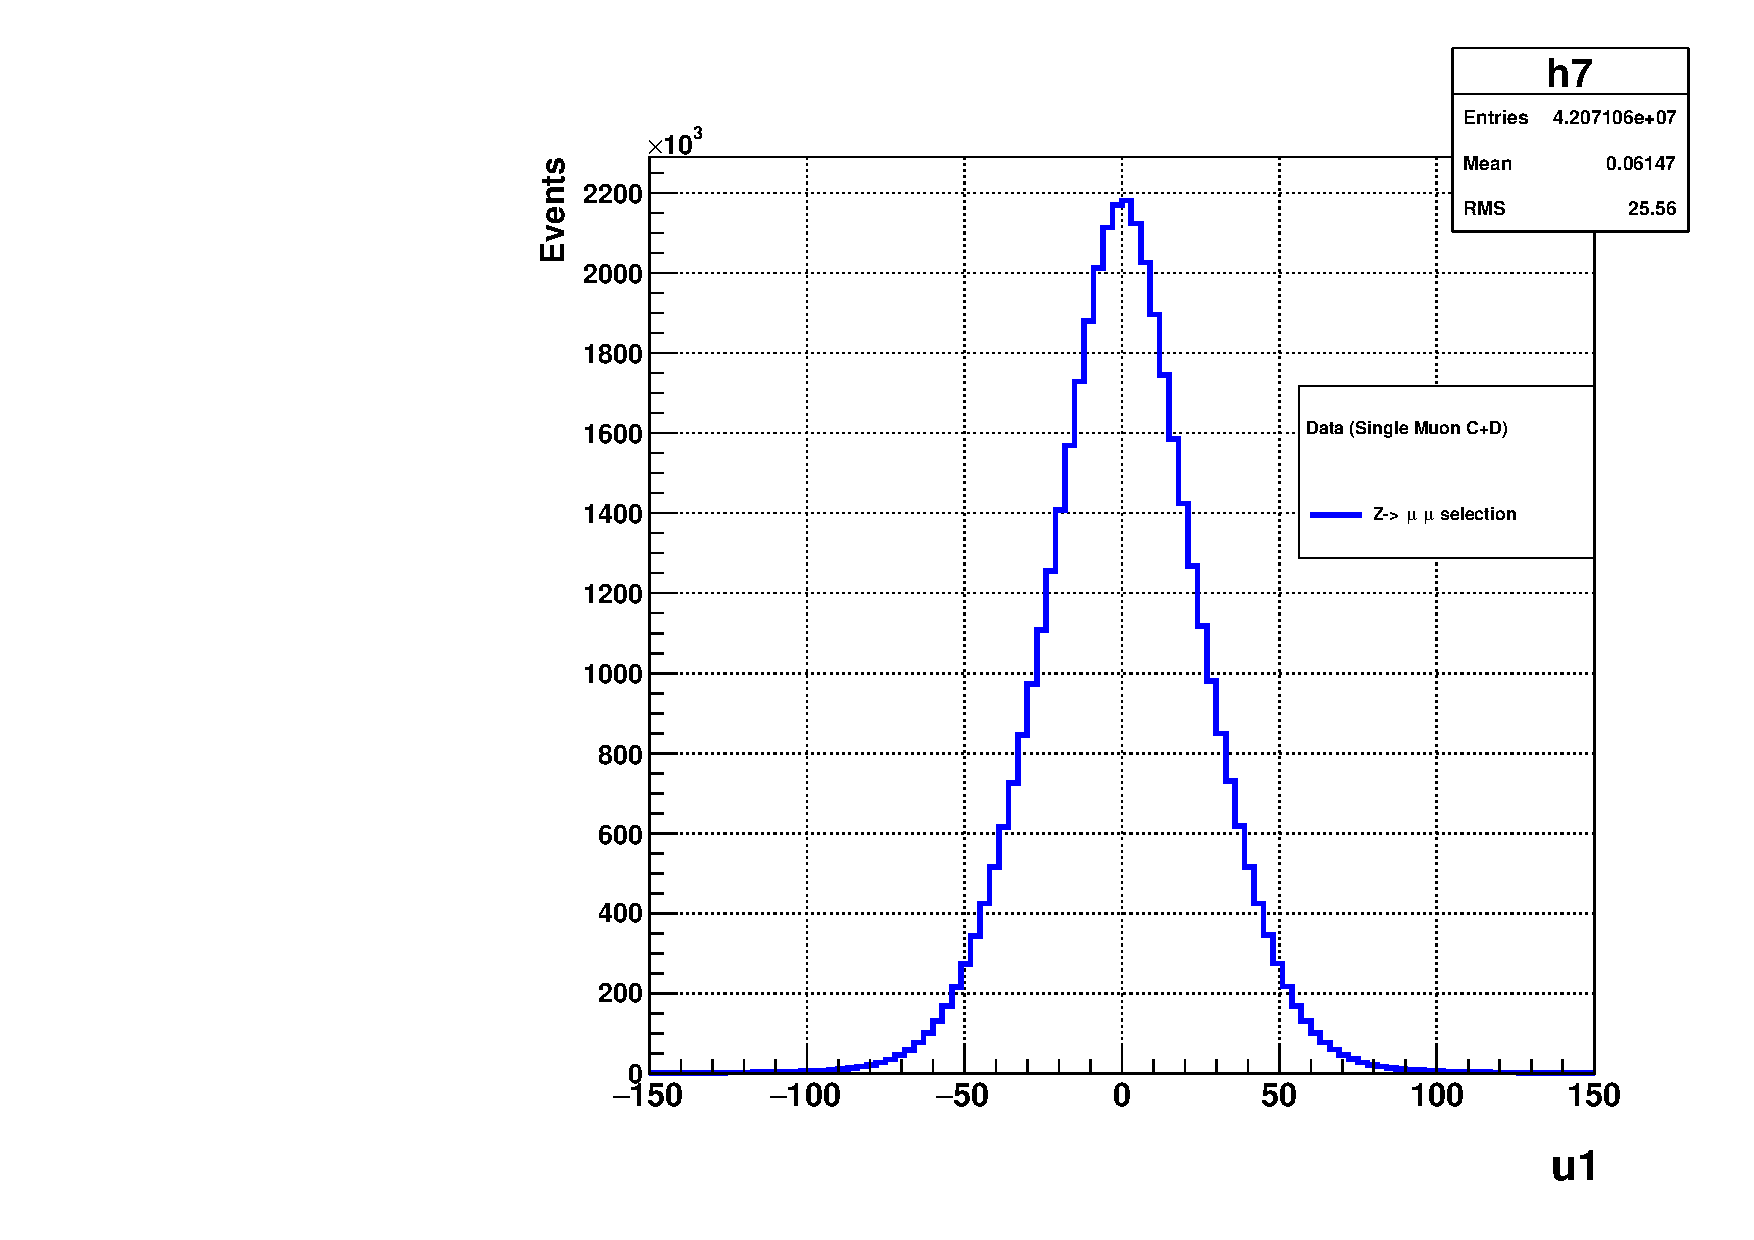
\includegraphics[width=180pt]{figuresARC/recoil/u1.pdf} &
  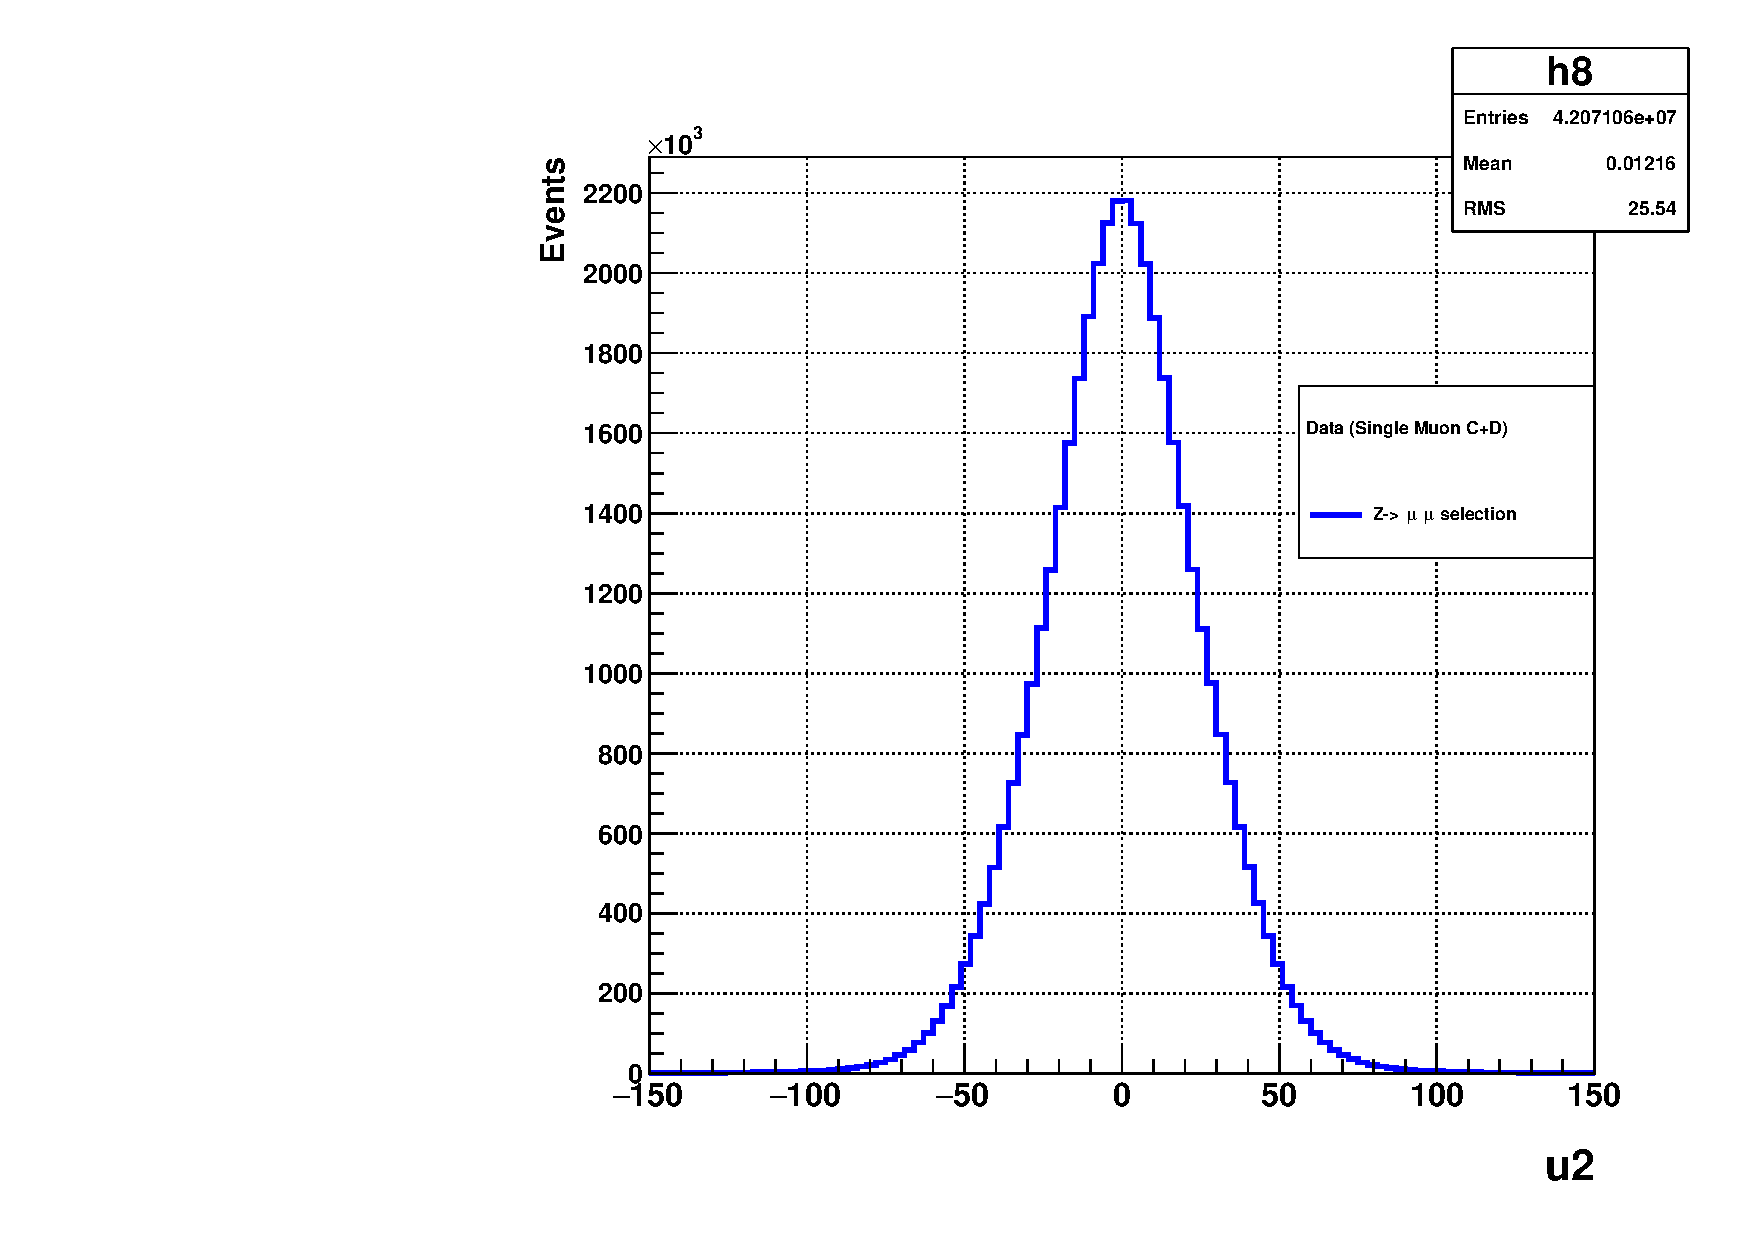
\includegraphics[width=180pt]{figuresARC/recoil/u2.pdf} \\
\end{tabular}
\begin{center}
  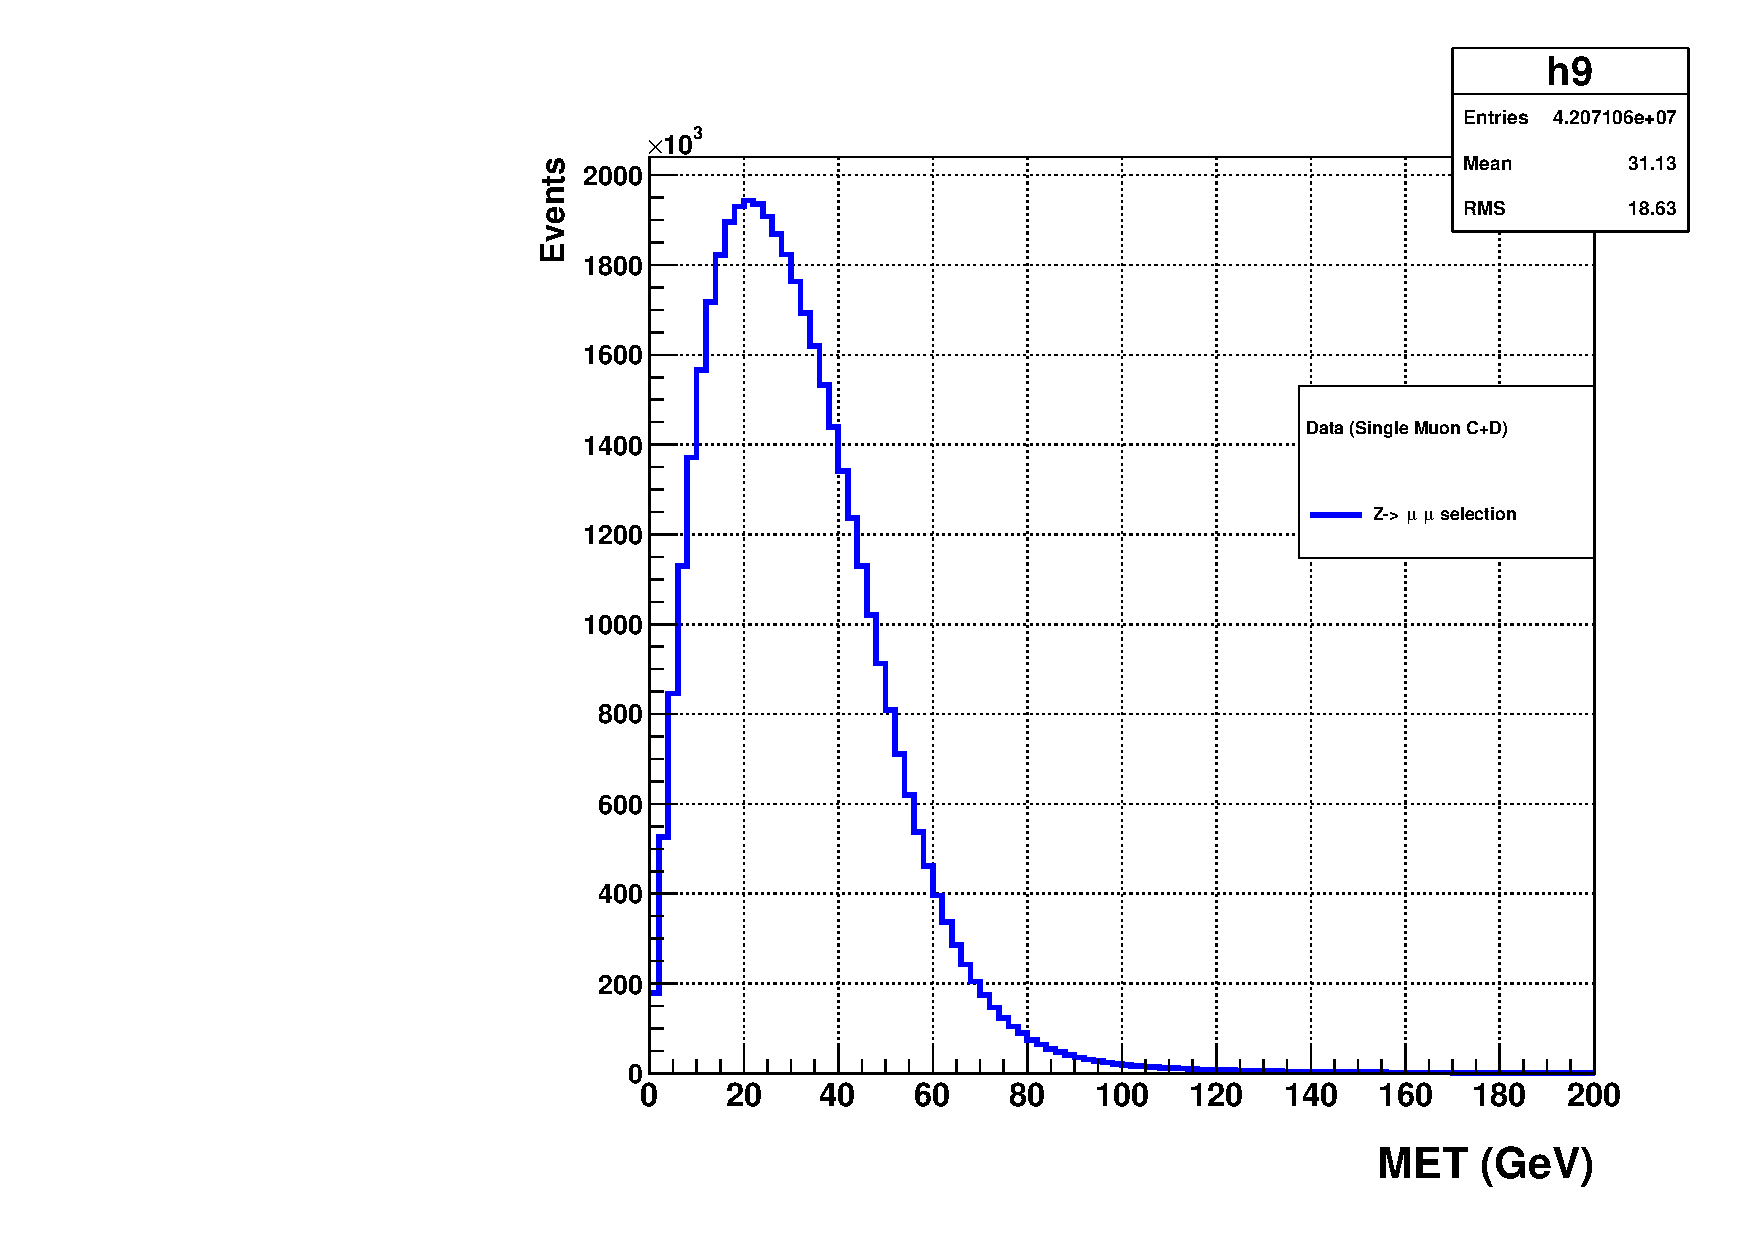
\includegraphics[width=200pt]{figuresARC/recoil/met.pdf}
\end{center}
\caption{Kinematic and recoil properties in the $Z \to \mu \mu$ process in Data after apply the selection .}
\label{fig:METrecoil1}
\end{figure}

\newpage
\begin{figure}[!ht]
\begin{tabular}{cc}
  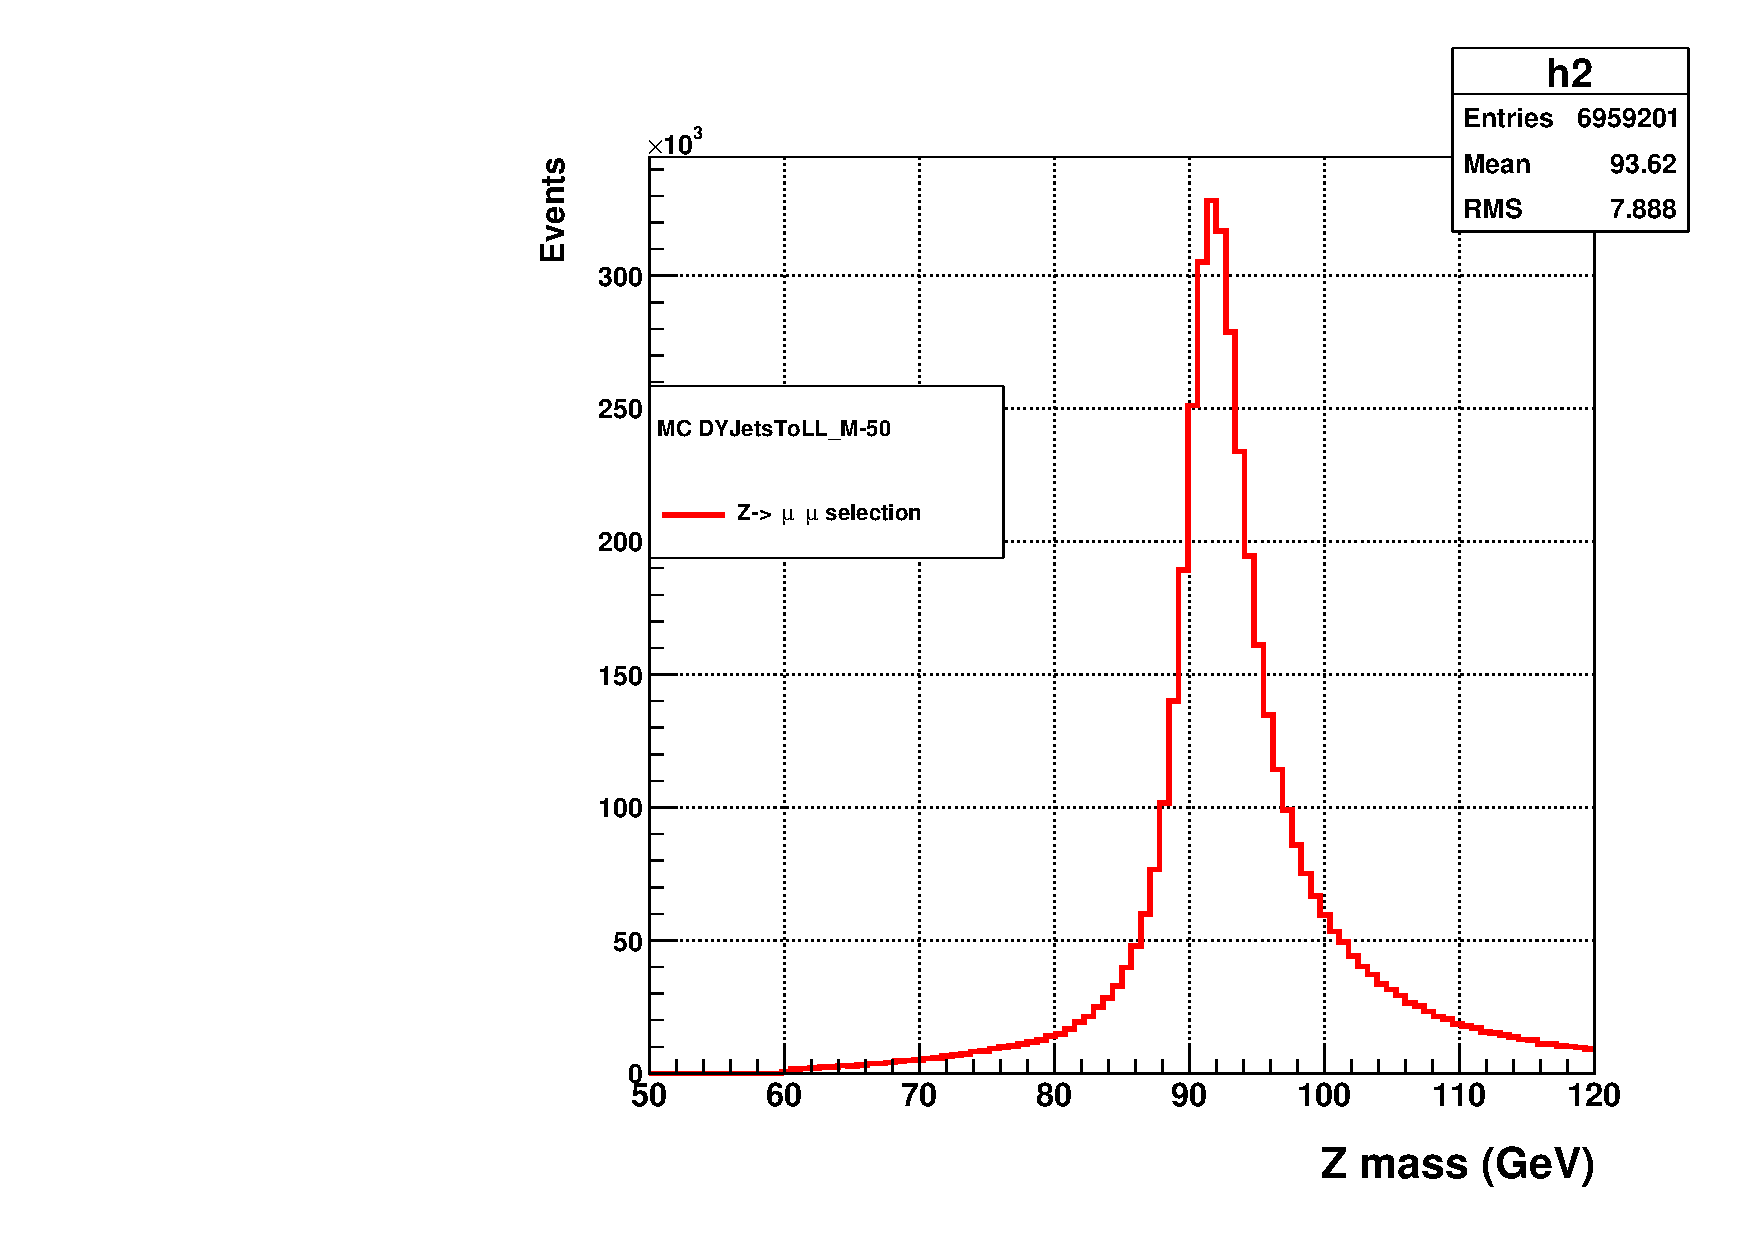
\includegraphics[width=180pt]{figuresARC/recoil/MC/dileptonMass.pdf} &
  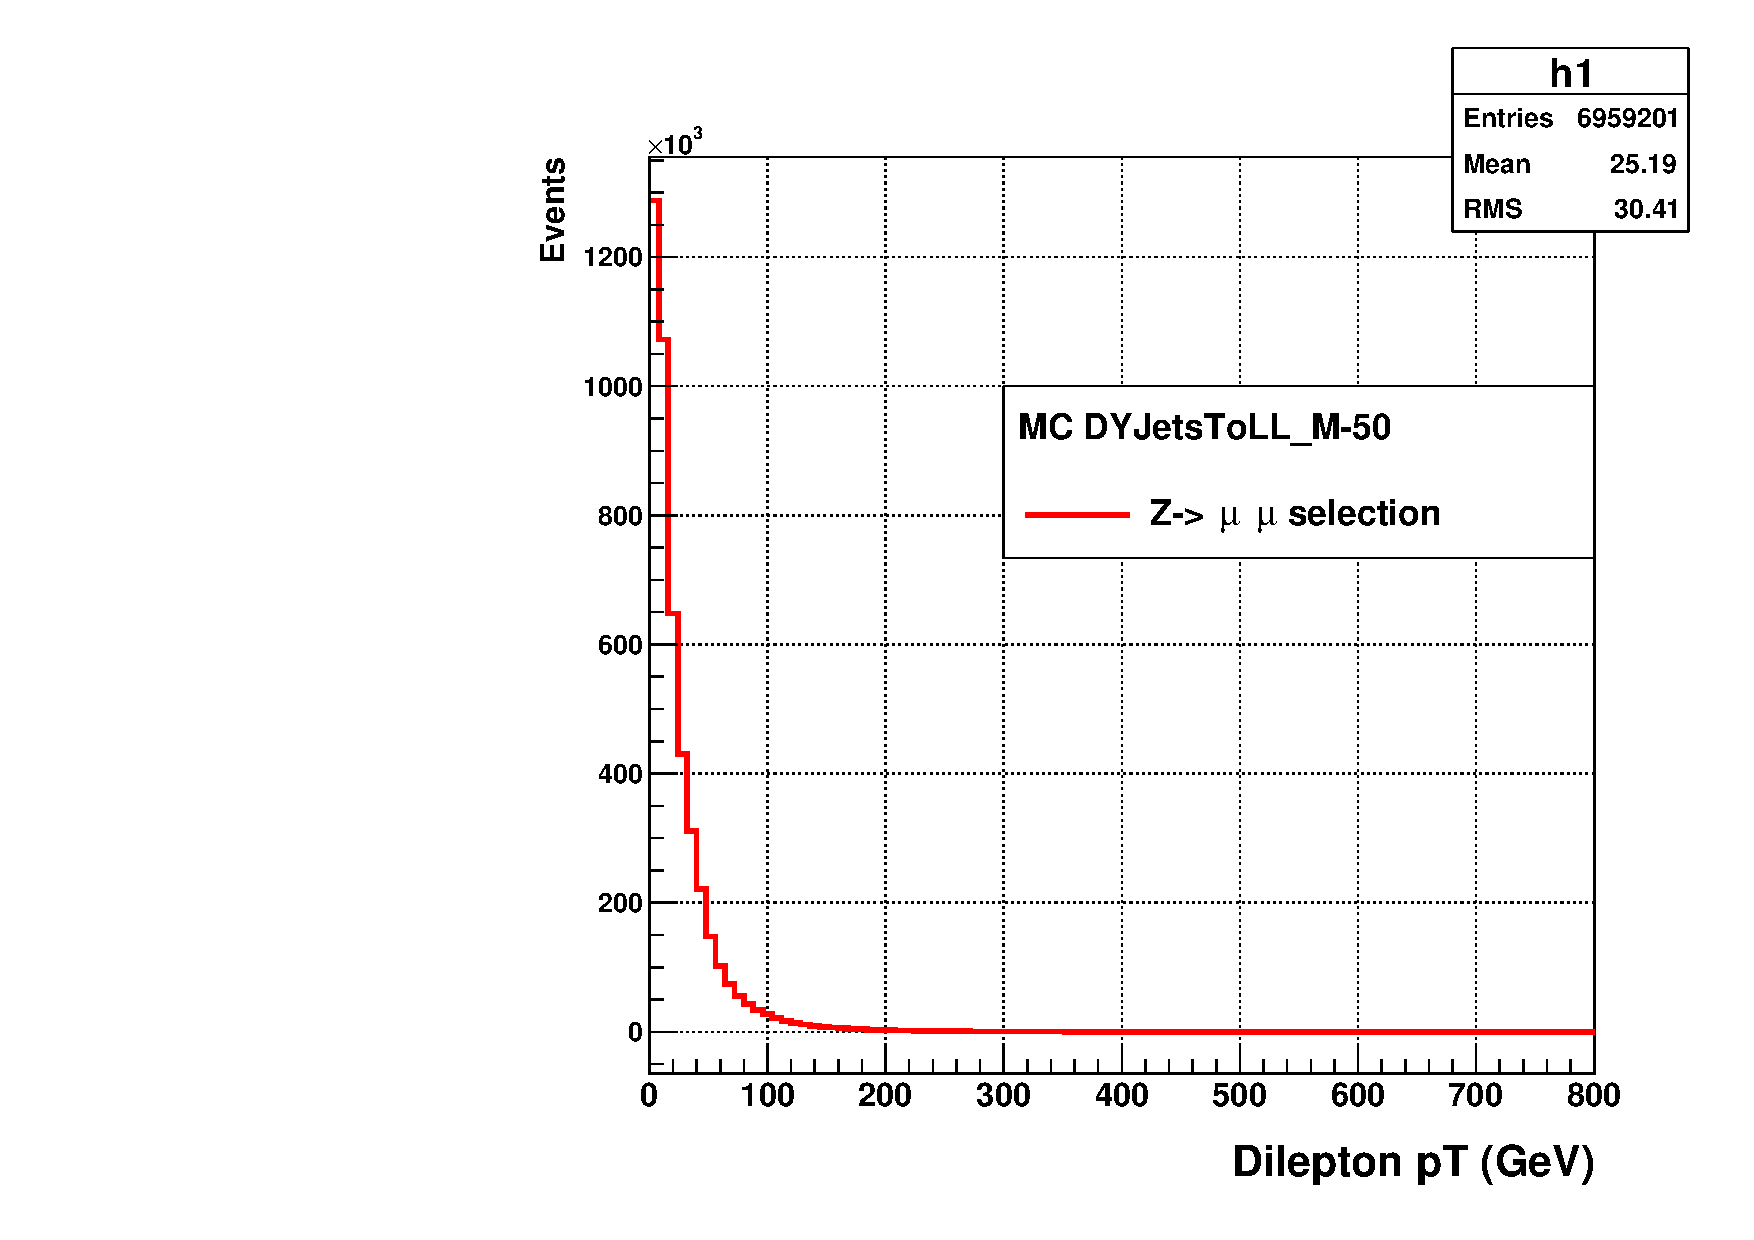
\includegraphics[width=180pt]{figuresARC/recoil//MC/dileptonpt.pdf} \\
  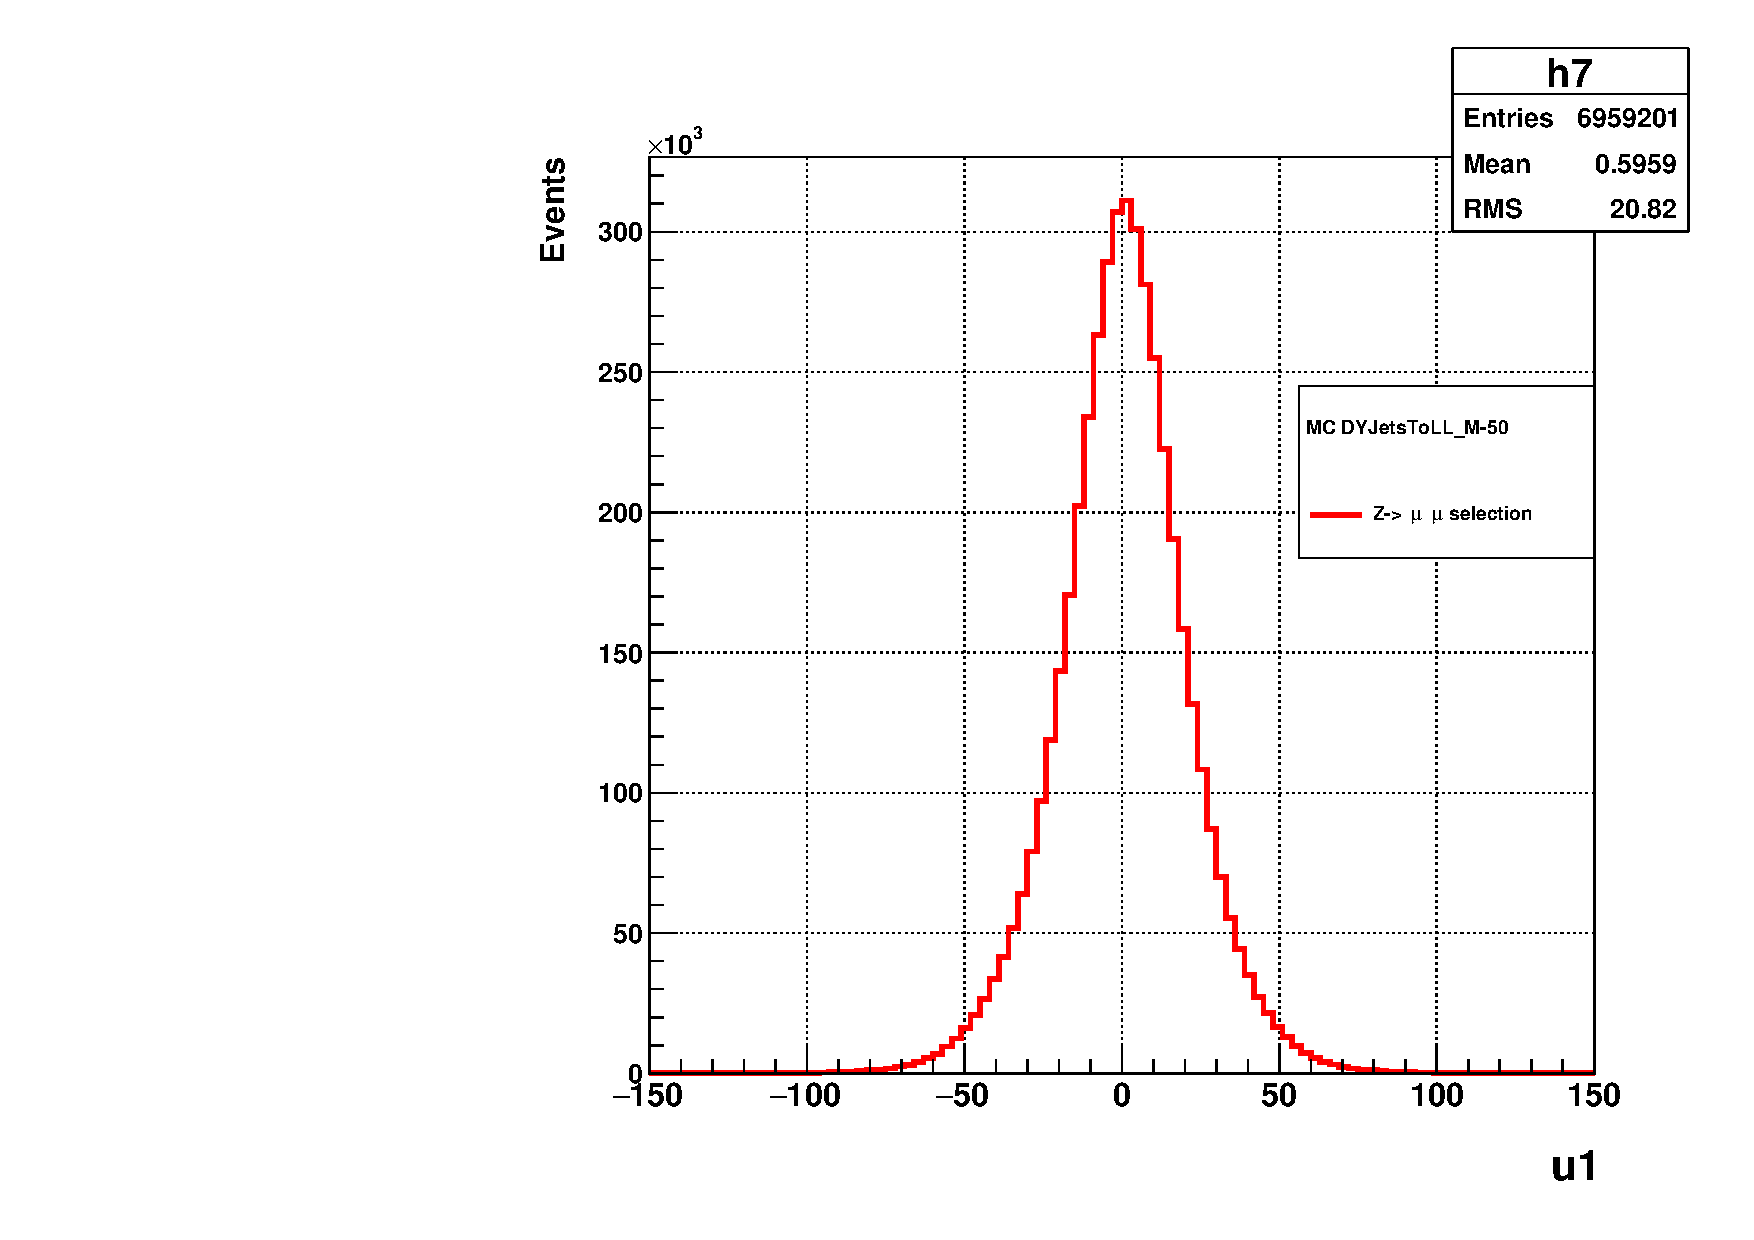
\includegraphics[width=180pt]{figuresARC/recoil/MC/u1.pdf} &
  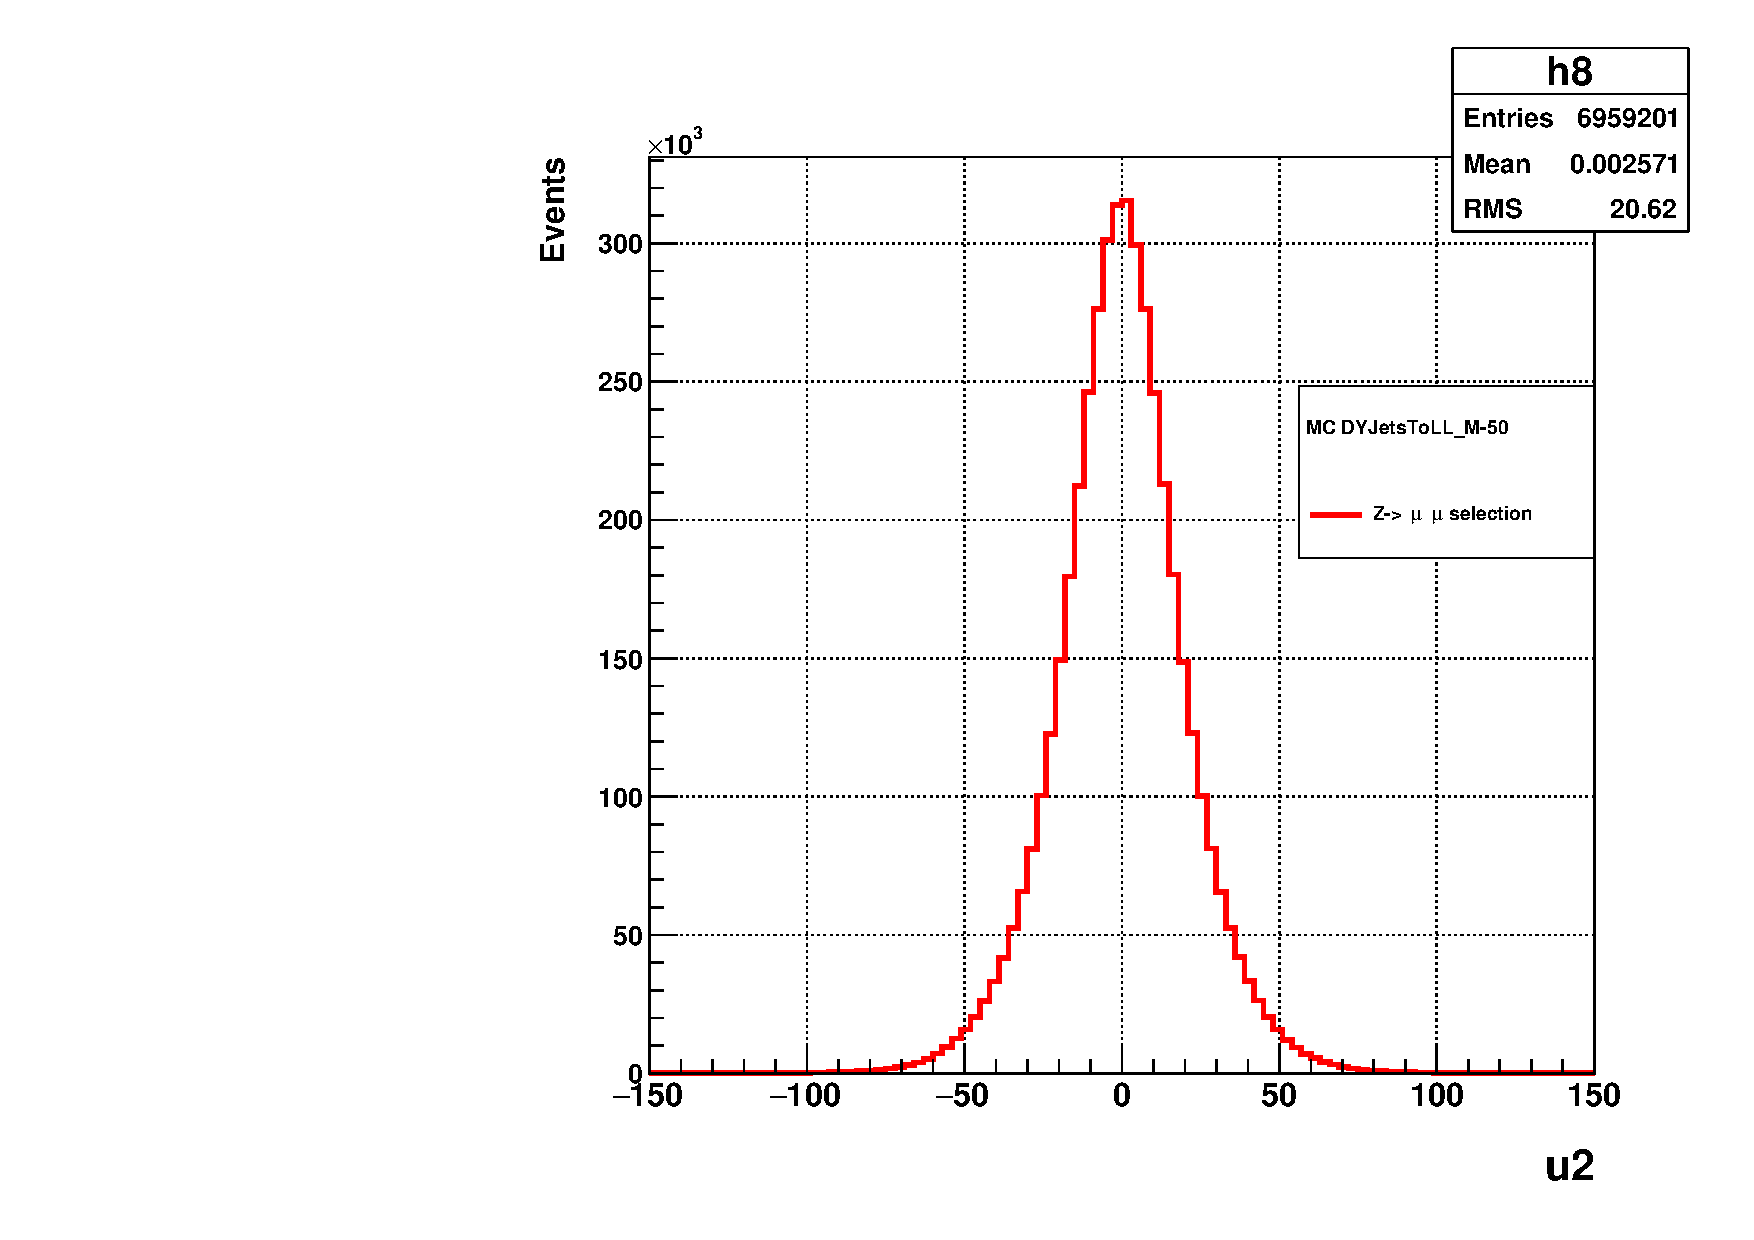
\includegraphics[width=180pt]{figuresARC/recoil/MC/u2.pdf} \\
\end{tabular}
\begin{center}
  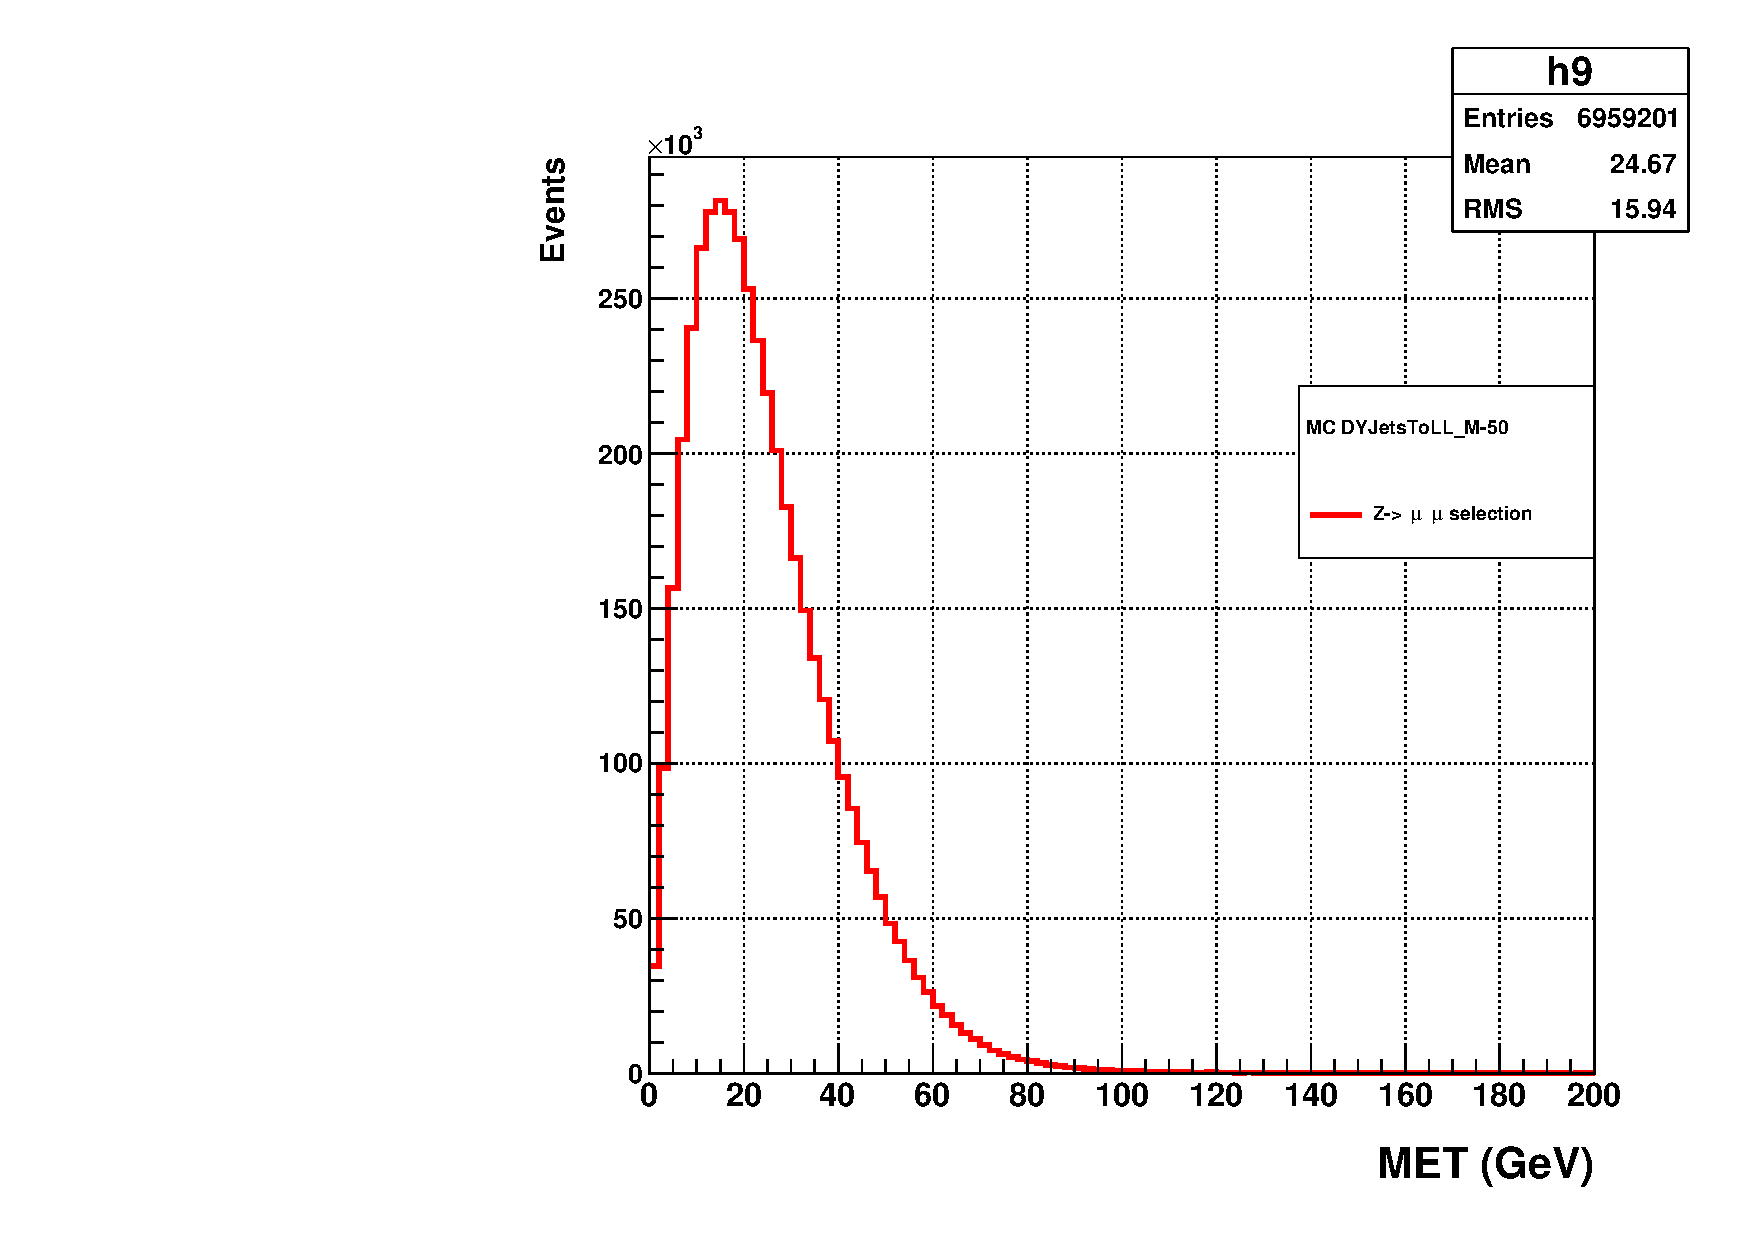
\includegraphics[width=200pt]{figuresARC/recoil/MC/met.pdf}
\end{center}
\caption{Kinematic and recoil properties in the $Z \to \mu \mu$ process in MC after apply the selection .}
\label{fig:METrecoil2}
\end{figure}

Figure \ref{fig:METrecoil3}, \ref{fig:METrecoil4}  shows the fit of the recoil in the parellel ($u_{1}$) and perpendicular ($u_{2}$) directions of the boson $\pt$ with a double gaussian model in different bins of the Z $\pt$.

\newpage
\begin{figure}[!ht]
\begin{tabular}{cccc}
  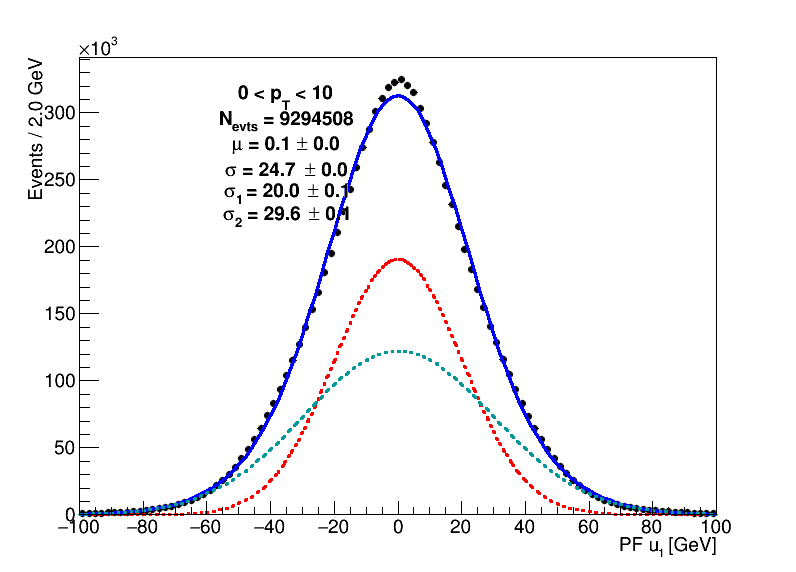
\includegraphics[width=100pt]{figuresARC/recoil/FITS/Data/pfu1fit_0.png} &
  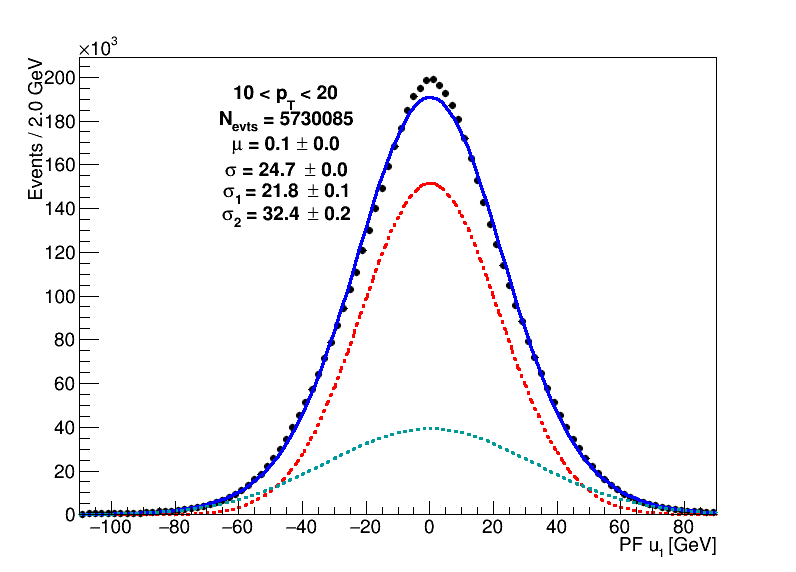
\includegraphics[width=100pt]{figuresARC/recoil/FITS/Data/pfu1fit_1.png} &
  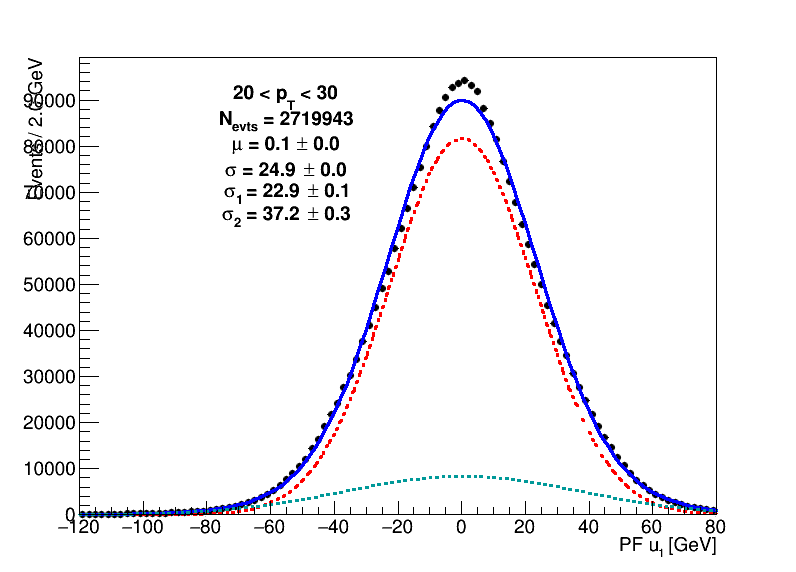
\includegraphics[width=100pt]{figuresARC/recoil/FITS/Data/pfu1fit_2.png} &
  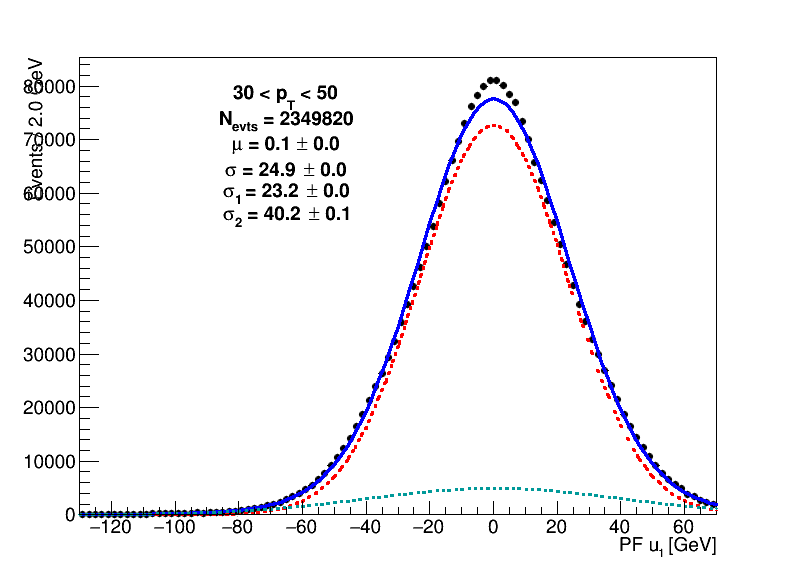
\includegraphics[width=100pt]{figuresARC/recoil/FITS/Data/pfu1fit_3.png} \\
  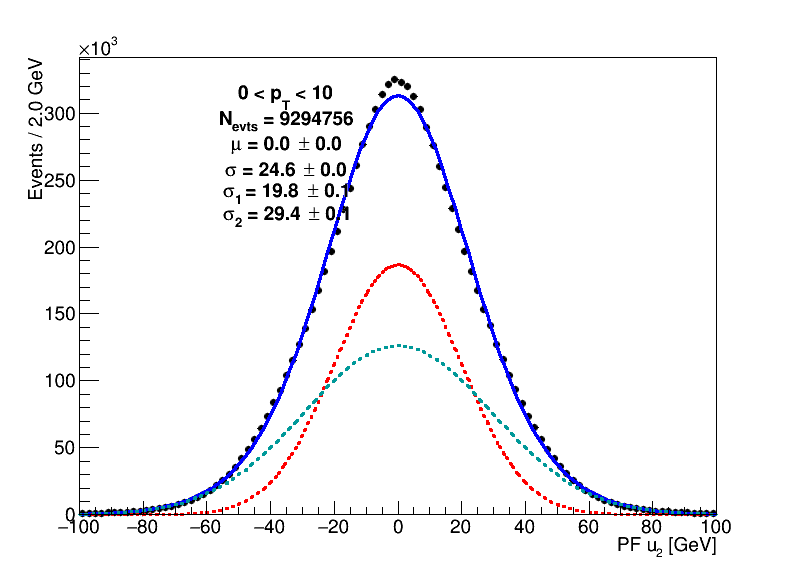
\includegraphics[width=100pt]{figuresARC/recoil/FITS/Data/pfu2fit_0.png} &
  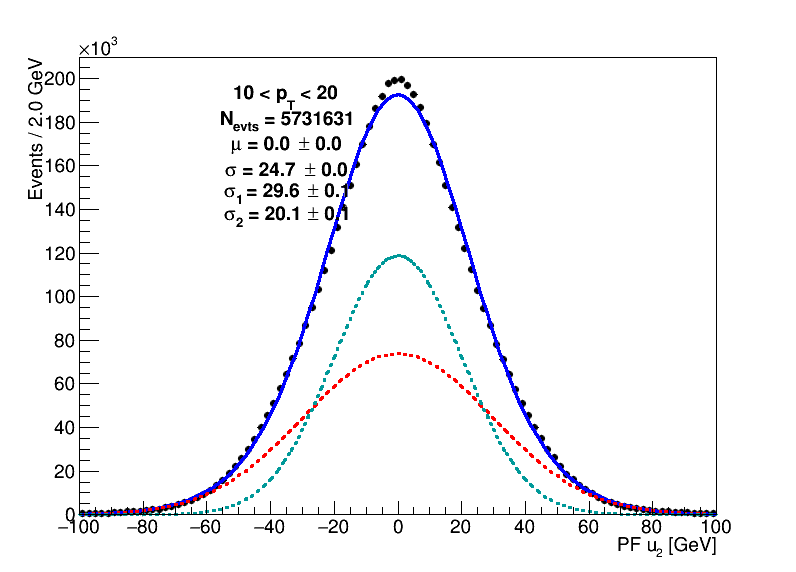
\includegraphics[width=100pt]{figuresARC/recoil/FITS/Data/pfu2fit_1.png} &
  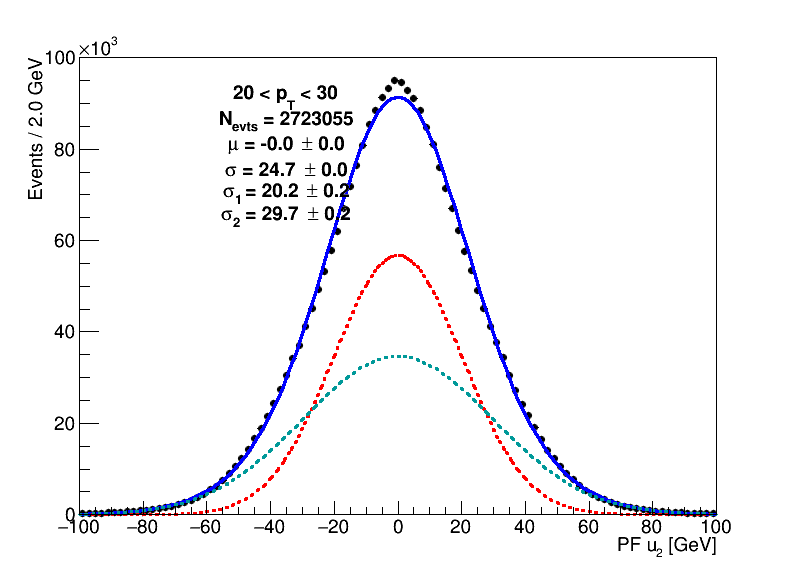
\includegraphics[width=100pt]{figuresARC/recoil/FITS/Data/pfu2fit_2.png} &
  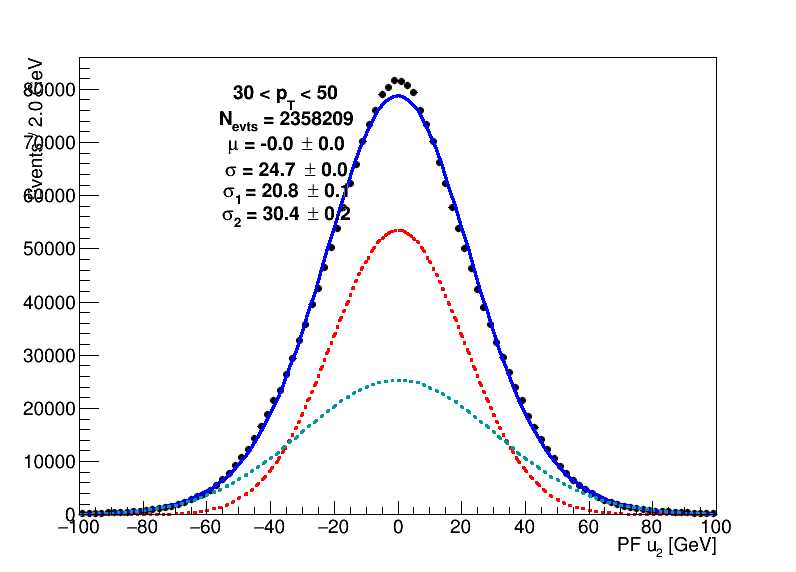
\includegraphics[width=100pt]{figuresARC/recoil/FITS/Data/pfu2fit_3.png} \\
\end{tabular}
\caption{Fits on the parallel ($u_{1}$) and perpendicular ($u_{2}$) components of the recoil in data with a double gaussian model.}
\label{fig:METrecoil3}
\end{figure}

\begin{figure}[!ht]
\begin{tabular}{cccc}
  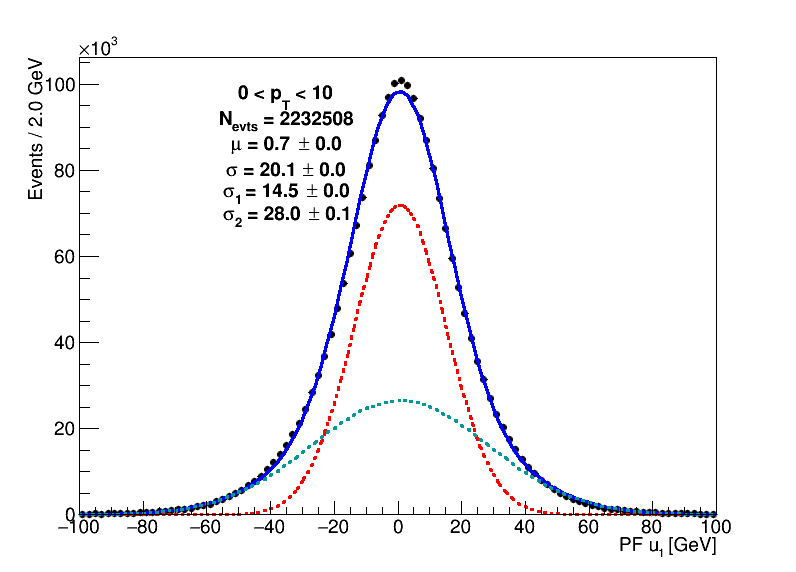
\includegraphics[width=100pt]{figuresARC/recoil/FITS/MC/pfu1fit_0.png} &
  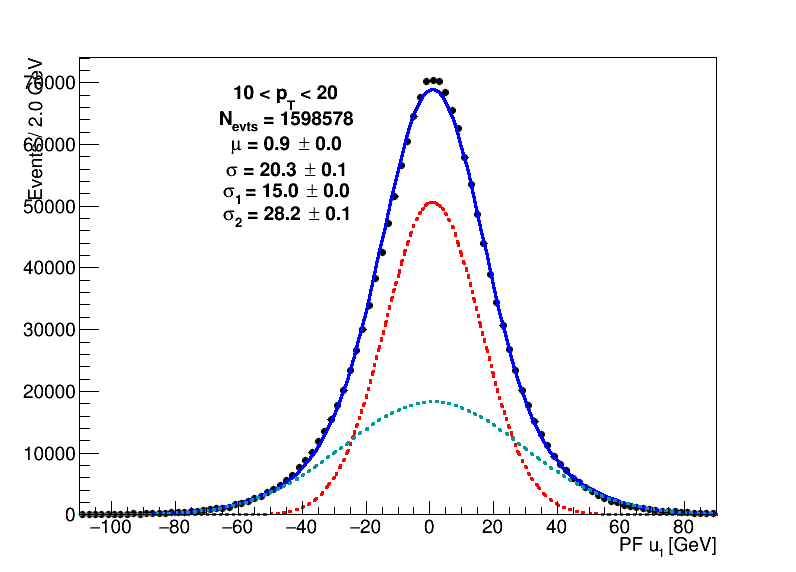
\includegraphics[width=100pt]{figuresARC/recoil/FITS/MC/pfu1fit_1MC.png} &
  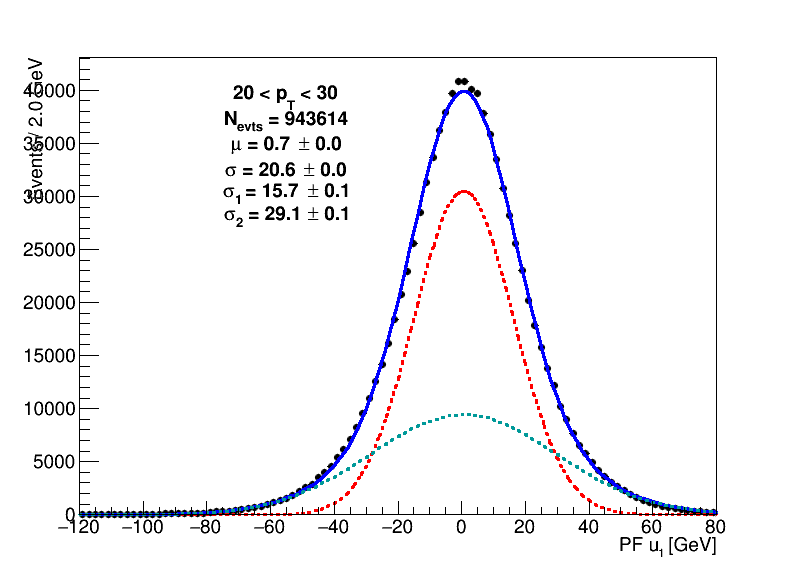
\includegraphics[width=100pt]{figuresARC/recoil/FITS/MC/pfu1fit_2.png} &
  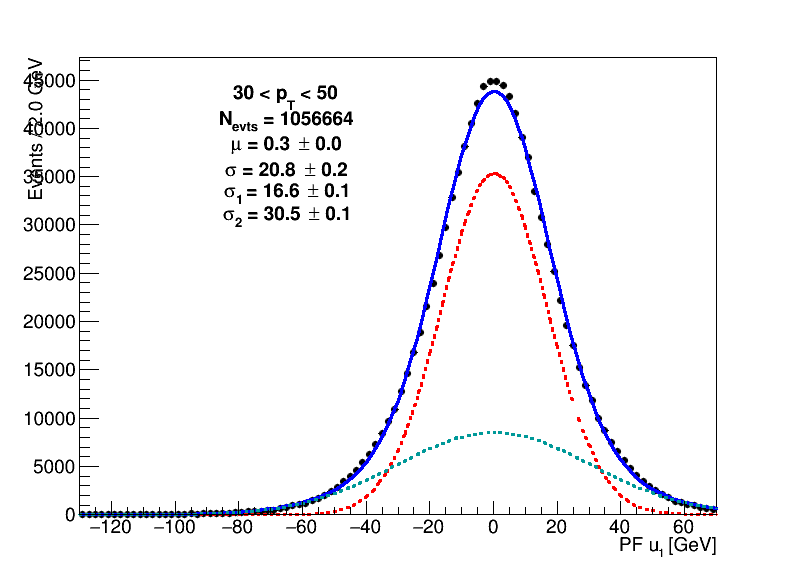
\includegraphics[width=100pt]{figuresARC/recoil/FITS/MC/pfu1fit_3.png} \\
  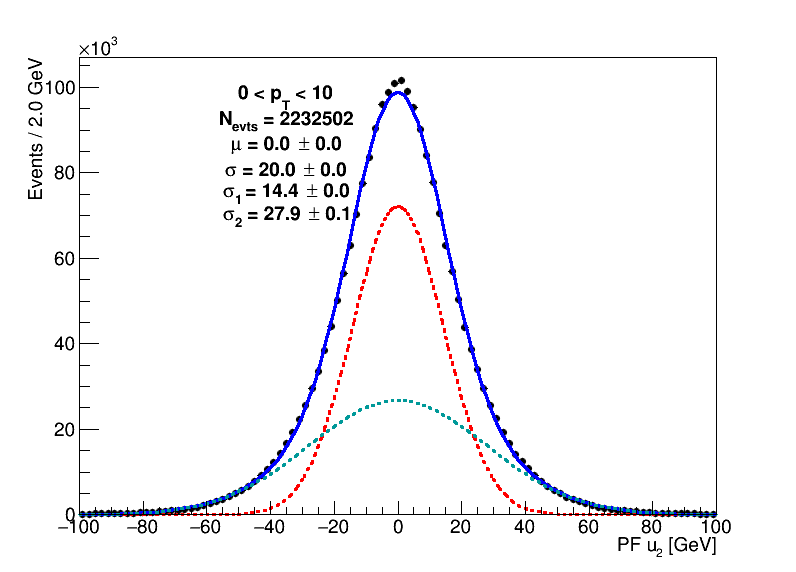
\includegraphics[width=100pt]{figuresARC/recoil/FITS/MC/pfu2fit_0.png} &
  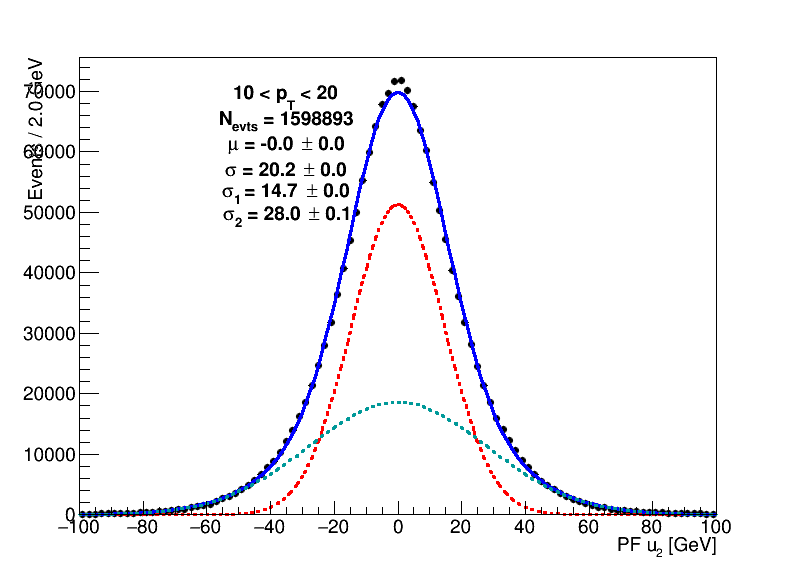
\includegraphics[width=100pt]{figuresARC/recoil/FITS/MC/pfu2fit_1MC.png} &
  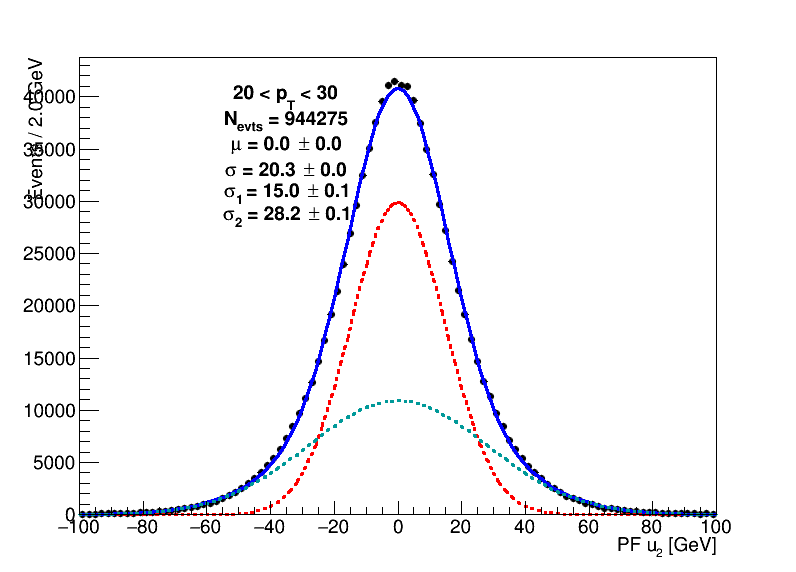
\includegraphics[width=100pt]{figuresARC/recoil/FITS/MC/pfu2fit_2.png} &
  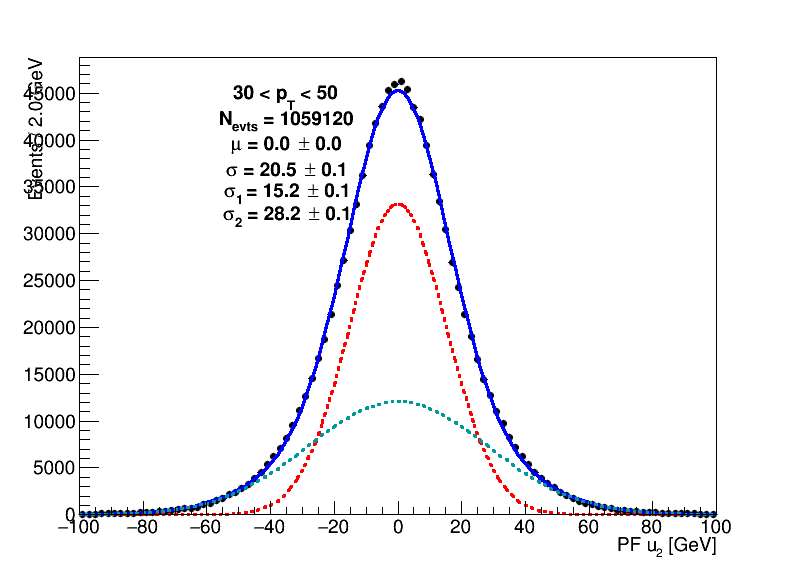
\includegraphics[width=100pt]{figuresARC/recoil/FITS/MC/pfu2fit_3.png} \\
\end{tabular}
\caption{Fits on the parallel ($u_{1}$) and perpendicular ($u_{2}$) components of the recoil in MC  with a double gaussian model}
\label{fig:METrecoil4}
\end{figure}

